\documentclass[tikz,border=10pt]{standalone}
% no extra libraries needed for a plain polygon
\begin{document}
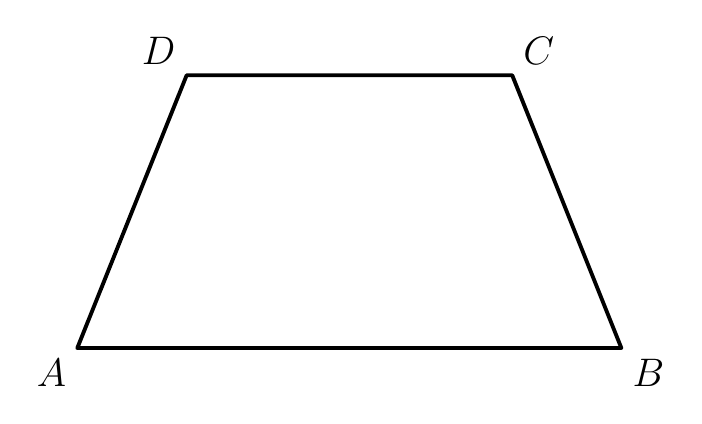
\begin{tikzpicture}[line width=1.4pt, line join=round]
% Vertices in cm: s = 0.017582 cm/px, centred on the ink bbox (cx=265.5, cy=144.5), y flipped
\coordinate (A) at (-3.4825,-1.7318);  % px (67.4,243.0)
\coordinate (B) at ( 3.4268,-1.7318);  % px (460.4,243.0)
\coordinate (C) at ( 2.0412, 1.7318);  % px (381.6,46.0)
\coordinate (D) at (-2.0940, 1.7318);  % px (146.4,46.0)

% Solid sides AB, BC, CD, DA, no fill
\draw (A) -- (B) -- (C) -- (D) -- cycle;

% Labels placed outside the figure (font from STYLE METRICS)
\node[below left]  at (A) {\fontsize{14.5}{17.4}\selectfont $A$};
\node[below right] at (B) {\fontsize{14.5}{17.4}\selectfont $B$};
\node[above right] at (C) {\fontsize{14.5}{17.4}\selectfont $C$};
\node[above left]  at (D) {\fontsize{14.5}{17.4}\selectfont $D$};
\end{tikzpicture}
\end{document}